% Part: sets-functions-relations
% Chapter: relations
% Section: graphs
% Hindi translation (hi-Deva-IN) of Open Logic commit 9620cc73f9c8e0ad003c514a5d3748f29611c4c0.

\documentclass[../../../include/open-logic-section]{subfiles}

\begin{document}

\olfileid[hi]{sfr}{rel}{grp}
\olsection{आलेख}

\emph{आलेख} ऐसा आरेख है जिसमें बिंदु---जिन्हें “संधि-बिंदु” या
“शीर्ष” कहते हैं---कोरों से जुड़े होते हैं। आलेख विविक्त गणित और संगणक
विज्ञान में सर्वत्र प्रयुक्त साधन हैं। संबंधों और संरचनाओं का निरूपण तथा
दृश्यांकन करने में वे अत्यंत उपयोगी हैं: विभिन्न प्रकार के संजाल जैसी मूर्त
वस्तुओं से लेकर निर्णयों के संभावित परिणाम जैसी अमूर्त संरचनाओं तक। साहित्य
में आलेखों के अनेक भिन्न प्रकार मिलते हैं। उदाहरण के लिए, वे इस बात के अनुसार
भिन्न होते हैं कि कोर दिष्ट हैं या नहीं, उन पर नामांक हैं या नहीं, किसी
संधि-बिंदु से उसी संधि-बिंदु तक कोर हो सकता है या नहीं, उन्हीं संधि-बिंदुओं
के बीच एकाधिक कोर हो सकते हैं या नहीं, आदि। \emph{दिष्ट आलेखों} का संबंधों
से विशेष नाता है।

\begin{defn}[दिष्ट आलेख]
\emph{दिष्ट आलेख} $G = \tuple{V, E}$ में \emph{शीर्षों} का एक
समुच्चय~$V$ और \emph{कोरों} का एक समुच्चय~$E \subseteq V^2$ होता है।
\end{defn}

\begin{explain}
हमारी परिभाषा के अनुसार आलेख बस एक समुच्चय और उस समुच्चय पर एक संबंध है।
निस्संदेह, आलेखों की चर्चा करते समय उनसे आलेखी रूप में निरूपित होने की अपेक्षा
स्वाभाविक है: हम दो शीर्षों~$v_1$ और $v_2$ को तीर से तभी और केवल तभी जोड़कर
आलेख बना सकते हैं जब $\tuple{v_1, v_2} \in E$। किसी संबंध और आलेख में एकमात्र
अंतर यह है कि आलेख शीर्षों के समुच्चय को स्पष्ट रूप से बताता है; अर्थात आलेख
में पृथक शीर्ष हो सकते हैं। फिर भी महत्त्वपूर्ण बात यह है कि हर संबंध~$R$ को,
जो समुच्चय~$X$ पर है, दिष्ट आलेख $\tuple{X, R}$ के रूप में देखा जा सकता है, और
इसके विपरीत दिष्ट आलेख~$\tuple{V, E}$ को संबंध $E \subseteq V^2$ के रूप में
देखा जा सकता है, जिसमें समुच्चय~$V$ स्पष्ट रूप से दिया गया है।
\end{explain}

\begin{ex}
आलेख $\tuple{V, E}$, जिसमें $V = \{1, 2, 3, 4\}$ और $E =
\{\tuple{1,1}, \allowbreak \tuple{1, 2}, \allowbreak \tuple{1, 3},
\allowbreak \tuple{2, 3}\}$ हैं, इस प्रकार दिखाई देता है:
\begin{align*}
& 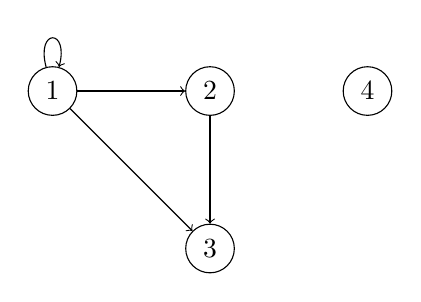
\begin{tikzpicture}[->,node distance=2cm]
  \node[draw,circle] (A) {$1$};
  \node[draw,circle] (B) [right of=A] {$2$};
  \node[draw,circle] (C) [below of=B] {$3$};
  \node[draw,circle] (D) [right of=B] {$4$};
  \draw (A) to [loop above]  (A);
  \draw (A) to  (B);
  \draw (A) to  (C);
  \draw (B) to  (C);
  \end{tikzpicture}
\intertext{यह उस $\tuple{V', E}$ से भिन्न आलेख है जिसमें $V' =
  \{1, 2, 3\}$ है और जो इस प्रकार दिखाई देता है:}
& 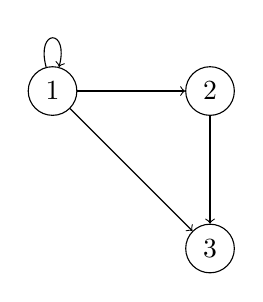
\begin{tikzpicture}[->,node distance=2cm]
  \node[draw,circle] (A) {$1$};
  \node[draw,circle] (B) [right of=A] {$2$};
  \node[draw,circle] (C) [below of=B] {$3$};
  \draw (A) to [loop above]  (A);
  \draw (A) to  (B);
  \draw (A) to  (C);
  \draw (B) to  (C);
  \end{tikzpicture}
\end{align*}
\end{ex}

\begin{prob}
  छोटा-या-बराबर संबंध~$\le$ को, जो समुच्चय $\{1,
  2, 3, 4\}$ पर है, आलेख के रूप में लीजिए और उसका संगत आरेख बनाइए।
\end{prob}

\end{document}
